\input{../../../headers/dsheaders.tex}

\section{Moteur Orthobloc 2000}

\begin{figure}[ht!]
\begin{minipage}{0.6\linewidth}
Le moteur Orthobloc 2000, figure \ref{ortho2000}, fait partie de la gamme des moto-reducteurs Leroy Somer. Il est constitué d'un bloc moteur qui transforme l'énergie électrique en mouvement de rotation (vitesse $\omega_{mot}$, couple $N_{mot}$) et d'un bloc réducteur dont la sortie est aussi un mouvement de rotation (vitesse $\omega_{red}$, couple $N_{red}$). Le rendement du réducteur est noté $\eta_{red}=0.9$.
\end{minipage}\hfill
\begin{minipage}{0.35\linewidth}
  \centering
  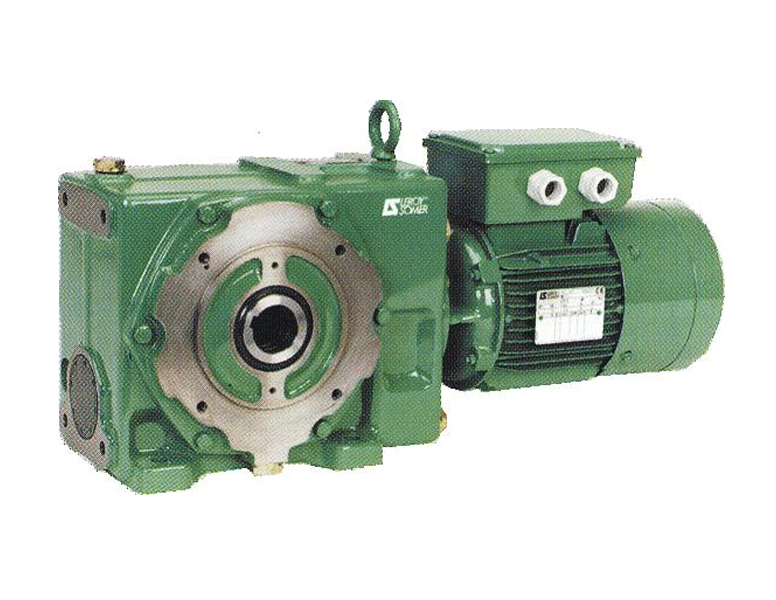
\includegraphics[width=\linewidth]{img/Orthobloc/photo}
  \caption{\label{ortho2000}Moteur Orthobloc 2000}
\end{minipage}
\end{figure}

Il est présentée en vue éclatée sur la figure \ref{ortho2000eclat}, avec la nomenclature associée sur la figure \ref{ortho2000nom}.

\begin{figure}[ht!]
 \centering
 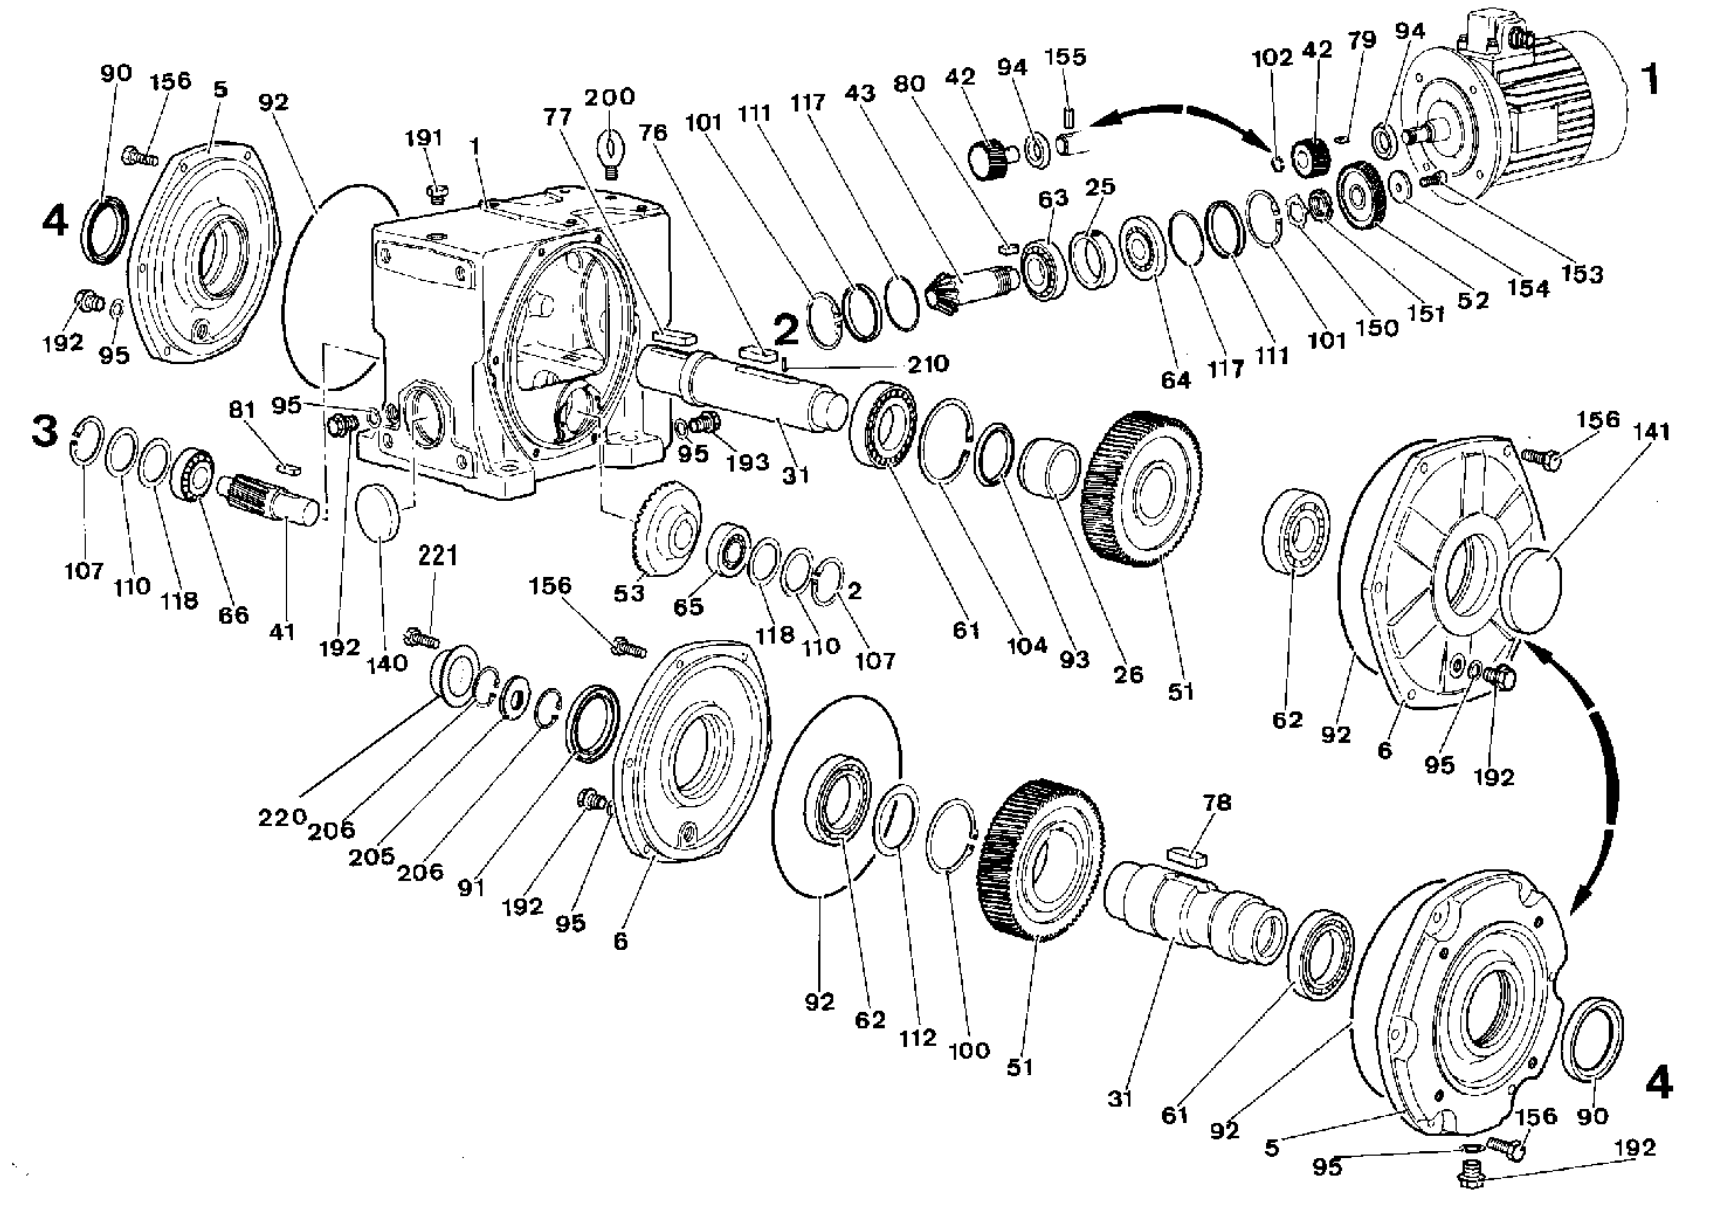
\includegraphics[width=\linewidth]{img/Orthobloc/eclat.png}
 \caption{\label{ortho2000eclat}Vue éclatée du moteur Orthobloc 2000}
\end{figure}

\begin{figure}[ht!]
 \centering
 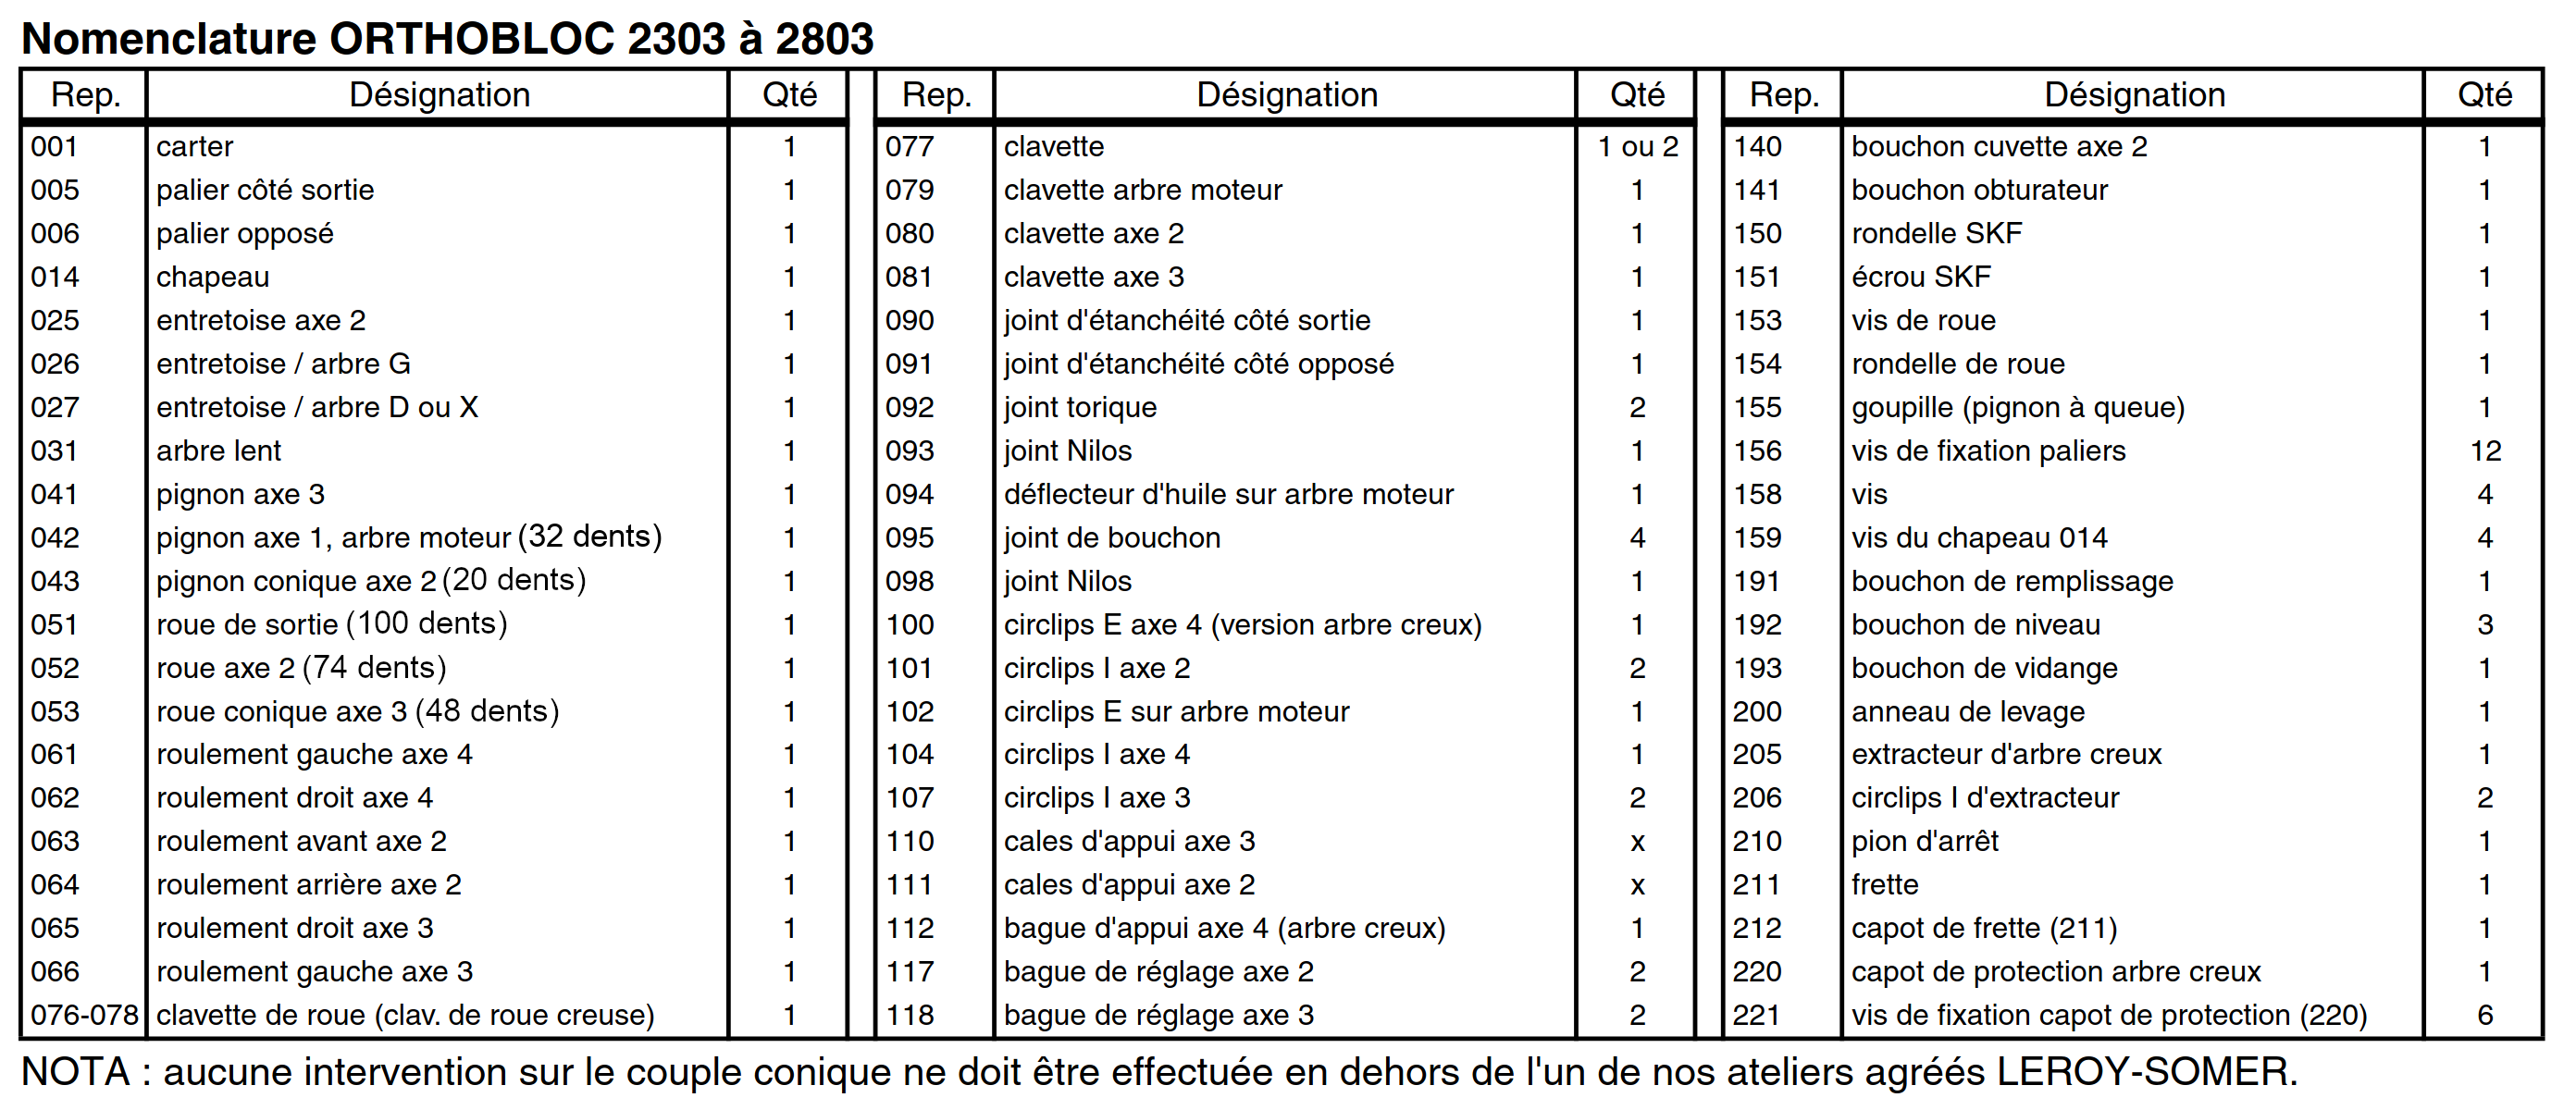
\includegraphics[width=\linewidth]{img/Orthobloc/nom.png}
 \caption{\label{ortho2000nom}Nomenclature du moteur Orthobloc 2000}
\end{figure}

\question{Compléter le dessin d'ensemble du document réponse, en intégrant les pièces 42, 43, 52, 79, 80, 102, 150, 151, 153, 154 et une partie de l'axe du rotor du motor. Une partie de ces pièces est présentée en vue projetée (l'échelle n'est pas celle du document réponse) sur la figure \ref{ortho2000pieces}.}

\begin{figure}[ht!]
 \centering
 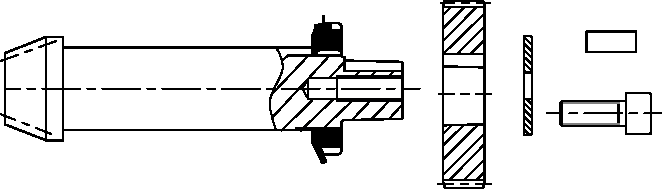
\includegraphics[width=\linewidth]{img/Orthobloc/pieces.pdf}
 \caption{\label{ortho2000pieces}Projection plane des pièces 43, 52, 80, 150, 151, 153, 154.}
\end{figure}

\question{Colorier sur le document réponse les cinq classes d'équivalence du moteur ainsi complété. Vous ferez attention à ce que le coloriage n'empêche pas la lisibilité du dessin de la question précédente.}

On nommera ces classes d'équivalence en fonction du numéro d'une des pièces de la classe d'équivalence. Par exemple, la classe d'équivalence incluant la pièce 001 sera appelée 1 et la classe contenant la pièce 031 sera appelée 31.

\question{Tracer le diagramme de liaisons du moteur, il faudra pour cela paramétrer le mécanisme (points, direction) afin que la modélisation des liaisons soient complètes.}

\newpage

Le formalisme à utiliser concernant les torseurs cinématiques pour la liaison entre les pièces i et j sera le suivant pour toute l'épreuve:
\begin{center}
$\left\{V_{i/j}\right\}=\left\{\begin{array}{cc}
\omega_{xij}&V_{xij}\\\omega_{yij}&V_{yij}\\\omega_{zij}&V_{zij}
\end{array}\right\}_{O,R}$
\end{center}

\question{Donner le torseur de la liaison pivot d'axe (A,$z_0$) entre les classes d'équivalence 1 et 31.}

\question{Donner les expressions et les valeurs numériques (à $10^-2$ près) des rapports $\dfrac{\omega_{red}}{\omega_{mot}}$ et $\dfrac{N_{red}}{N_{mot}}$.}

\section{Pelleteuse}

Le schéma cinématique d'une pelleteuse hydraulique est présenté à la figure \ref{pelleteuse_cin}.

\begin{figure}[ht!]
 \def\svgwidth{.8\linewidth}
 \input{img/Pelleteuse/schema_cinematique.pdf_tex}
 \caption{\label{pelleteuse_cin}Schéma cinématique paramétré de la pelleteuse}
\end{figure}

Données géométriques:
\begin{itemize}
 \item $\overrightarrow{AC}=l_{910}\cdot \overrightarrow{x_9}$
 \item $\overrightarrow{DF}=l_{78}\cdot \overrightarrow{x_7}$
 \item $\overrightarrow{GH}=l_{45}\cdot \overrightarrow{x_4}$
 \item $\overrightarrow{DE}=a\cdot \overrightarrow{x_{11}}-b\cdot \overrightarrow{y_{11}}$
 \item $\overrightarrow{EJ}=c\cdot \overrightarrow{x_6}$
\end{itemize}

De plus, dans le cadre de notre étude, il sera supposé que $(\overrightarrow{x_7},\overrightarrow{x_{11}})=(\overrightarrow{y_7},\overrightarrow{y_{11}})=0$.

\question{Tracer le graphe de liaisons de la pelleteuse.}

\question{Écrire les torseurs $\left\{V_{6/11}\right\}$, $\left\{V_{6/7}\right\}$, $\left\{V_{7/8}\right\}$ et $\left\{V_{8/11}\right\}$ respectivement aux points E, F, D et D, dans la base $R_7$.}

\question{Écrire les torseurs $\left\{V_{6/11}\right\}$ et $\left\{V_{6/7}\right\}$ au point D dans la base $R_7$.}

\question{A l'aide d'une fermeture cinématique issue du cycle du graphe de liaison et qui intègre les torseurs précédemment déterminés, établir un système de 6 équations cinématiques.}

\question{Déterminer alors $\omega_{x78}$.}

\question{Déterminer la norme du vecteur $\overrightarrow{\Omega_{6/11}}$ en fonction de la vitesse de sortie du vérin 7/8.}

\question{Déterminer $\overrightarrow{V_{J\in 6/11}}$, en fonction de la vitesse de sortie du vérin 7/8 et des paramètres géométrique du système, dans la base $R_6$.}

\section{Rotor d'hélicoptère}

La boite de transmission, figure \ref{helico2}, est l'organe qui transmet le couple généré par le moteur aux pales de l'hélicoptère, figure \ref{helico1}.

\begin{figure}[ht!]
\begin{minipage}{0.45\linewidth}
 \centering
 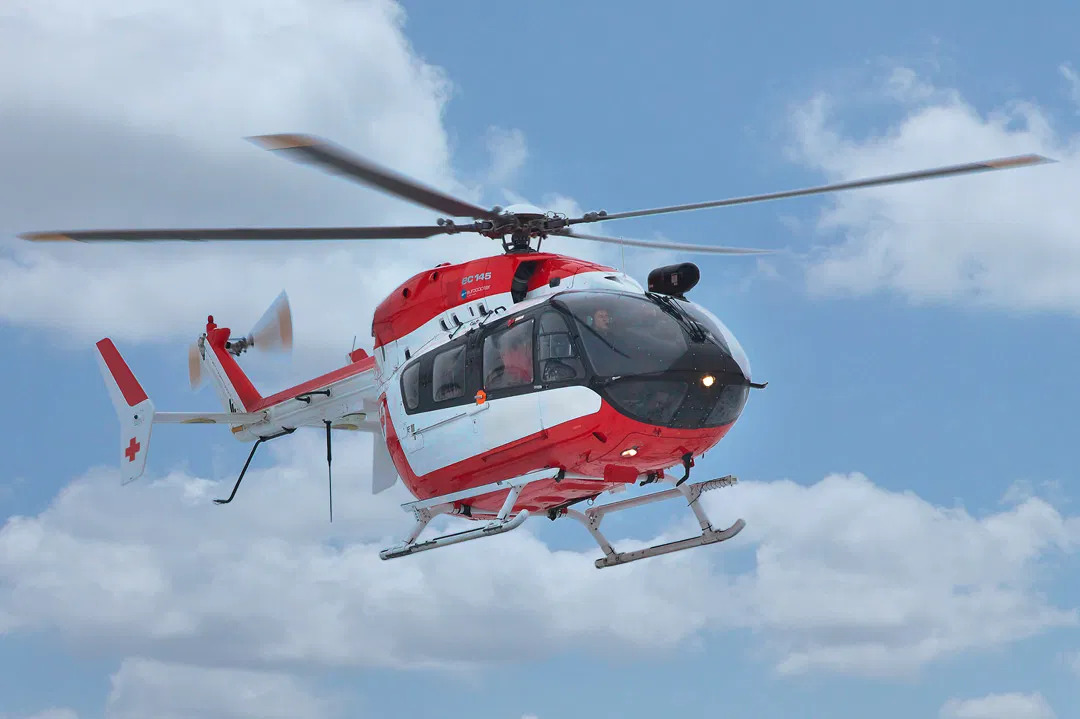
\includegraphics[width=\linewidth]{img/Hélico/photo1}
 \caption{\label{helico1}Hélicoptère}
\end{minipage}\hfill
\begin{minipage}{0.45\linewidth}
 \centering
 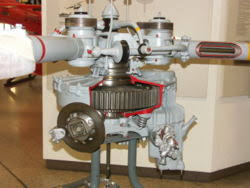
\includegraphics[width=\linewidth]{img/Hélico/photo2}
 \caption{\label{helico2}Boite de transmission ouverte d'un hélicoptère}
\end{minipage}\hfill
\end{figure}

Le dessin d'ensemble d'une boite de transmission est donné sur le document réponse.

\question{Colorier les 5 classes d'équivalence de la boite de transmission du rotor d'hélicoptère.}

\question{Tracer le graphe de liaisons de la boite de transmission du rotor d'hélicoptère. Il faudra pour cela ajouter sur le document réponse de la question précédente, les directions et les points nécessaires à la définition des liaisons.}

\question{Tracer le schéma cinématique paramétré de la boite de transmission du rotor d'hélicoptère.}

Soit $\omega_{mot}$ la vitesse de rotation du moteur de l'hélicoptère et $\omega_{pal}$ la vitesse de rotation des pales.

\question{Déterminer le rapport $\dfrac{\omega_{pal}}{\omega_{mot}}$.}

%\finsujet{public}
\finsujet

\def\public
\sautpage{3}
\debutcor

\reponse[2]{0}{Voir plan A3.
}{\begin{center}
 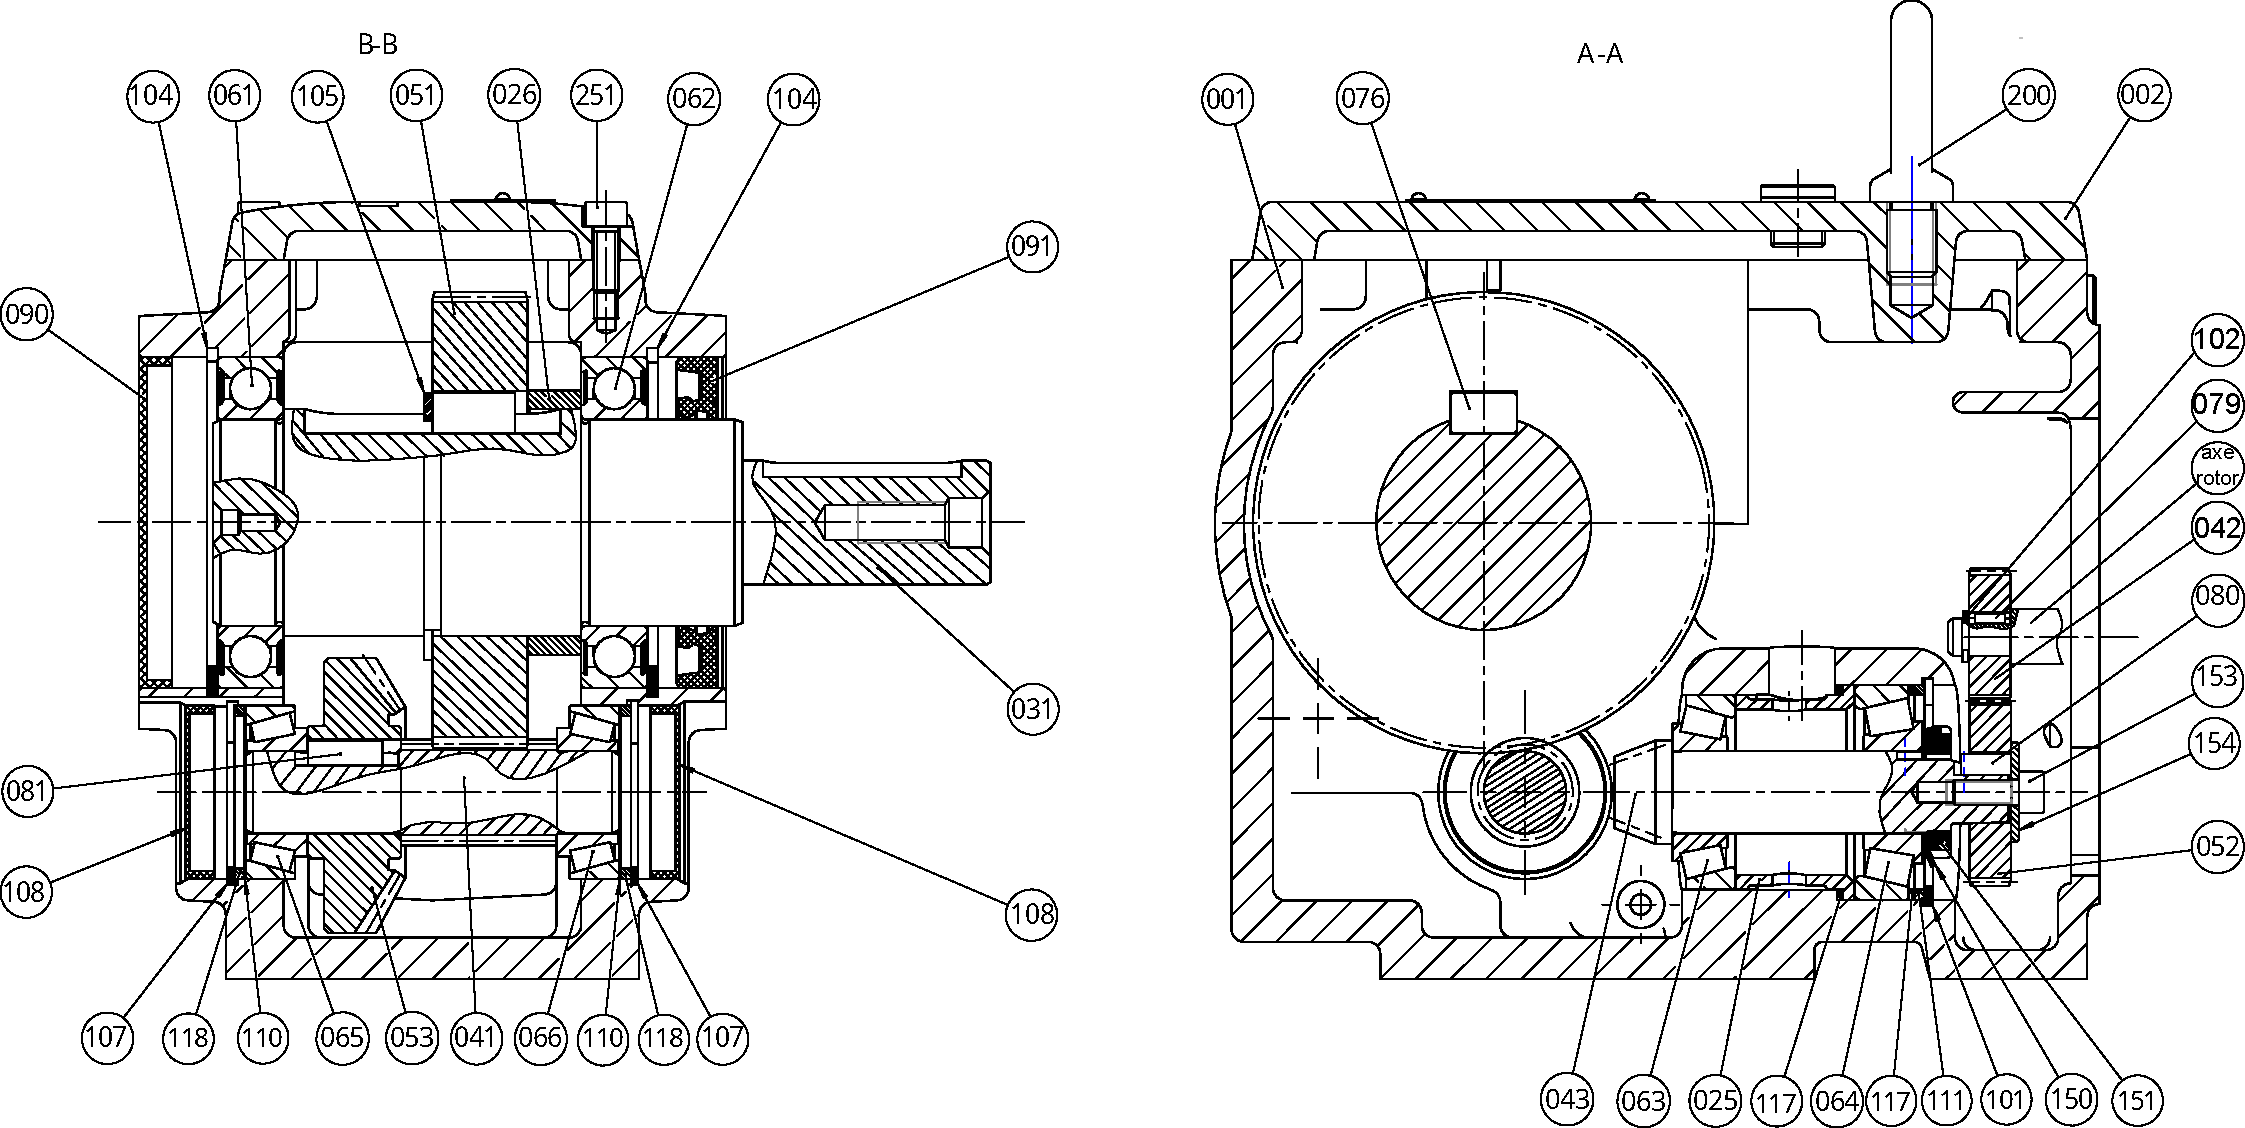
\includegraphics[width=\linewidth]{img/Orthobloc/plan_cor.pdf} \\ 
  \def\svgwidth{.8\linewidth}
 \input{img/Orthobloc/plan_col_cor.pdf_tex}
 \end{center}
}

\reponse{8}{}{\begin{center}
 \def\svgwidth{.8\linewidth}
 \input{img/Orthobloc/graphe_liaisons.pdf_tex}
\end{center}}

\reponse{2}{}{
$\left\{V_{31/1}\right\}=\left\{\begin{array}{cc}
0&0\\0&0\\\omega_{z311}&0
\end{array}\right\}_{A,R}$
}
   
\reponse{6}{}{
$\dfrac{\omega_{red}}{\omega_{mot}}=\dfrac{Z_{42}\cdot Z_{43}\cdot Z_{51}}{Z_{52}\cdot Z_{53}\cdot Z_{51}}$

$\dfrac{\omega_{red}}{\omega_{mot}}=\dfrac{32\cdot 20}{74\cdot 48}=\dfrac{4\cdot 5}{37\cdot 3}=\dfrac{20}{111}=\dfrac{22,2}{111}-\dfrac{2,2}{111}=0,2-0,02)=0,18$

$\dfrac{N_{red}}{N_{mot}}=0.9\cdot \dfrac{111}{20}=\dfrac{99.9}{20}\approx 5$
}

\reponse{8}{}{
 \def\svgwidth{.8\linewidth}
 \input{img/Pelleteuse/graphe_liaisons.pdf_tex}
}


\reponse{6}{}{
$\left\{V_{6/11}\right\}=\left\{\begin{array}{cc}
0&0\\0&0\\\omega_{z611}&0
\end{array}\right\}_{E,R_7}$

$\left\{V_{6/7}\right\}=\left\{\begin{array}{cc}
0&0\\0&0\\\omega_{z67}&0
\end{array}\right\}_{F,R_7}$

$\left\{V_{7/8}\right\}=\left\{\begin{array}{cc}
\omega_{x78}&V_{x78}\\0&0\\0&0
\end{array}\right\}_{D,R_7}$

$\left\{V_{8/11}\right\}=\left\{\begin{array}{cc}
0&0\\0&0\\\omega_{z811}&0
\end{array}\right\}_{D,R_7}$
}

\reponse{6}{}{
$\left\{V_{6/11}\right\}=\left\{\begin{array}{cc}
0&0\\0&0\\\omega_{z611}&0
\end{array}\right\}_{E,R_7}=\left\{\begin{array}{cc}
0&-b\cdot \omega_{z611}\\0&-a\cdot \omega_{z611}\\\omega_{z611}&0
\end{array}\right\}_{D,R_7}$

$\left\{V_{6/7}\right\}=\left\{\begin{array}{cc}
0&0\\0&0\\\omega_{z67}&0
\end{array}\right\}_{F,R_7}=\left\{\begin{array}{cc}
0&0\\0&-l_{78}\cdot \omega_{z67}\\\omega_{z67}&0
\end{array}\right\}_{D,R_7}$

$\left\{V_{7/8}\right\}=\left\{\begin{array}{cc}
\omega_{x78}&V_{x78}\\0&0\\0&0
\end{array}\right\}_{D,R_7}$

$\left\{V_{8/11}\right\}=\left\{\begin{array}{cc}
0&0\\0&0\\\omega_{z811}&0
\end{array}\right\}_{D,R_7}$
}

\reponse{6}{}{La fermeture cinématique implique:\\
$\left\{V_{6/11}\right\}=\left\{V_{6/7}\right\}+\left\{V_{7/8}\right\}+\left\{V_{8/11}\right\}$

Le système ainsi obtenu est alors:\\
$\left\{\begin{array}{l}
0=0+\omega_{x78}+0\\
0=0+0+0\\
\omega_{z611}=\omega_{z67}+0+\omega_{z811}\\
-b\cdot \omega_{z611}=0+V_{x78}+0\\
-a\cdot \omega_{z611}=-l_{78}\cdot \omega_{z67}+0+0\\
0=0+0+0\\
\end{array}\right.$}

\reponse{3}{}{$\omega_{x78}=0$}

\reponse{3}{}{$\omega_{z611}=-\dfrac{V_{x78}}{b}$}

\reponse{4}{}{$\overrightarrow{V_{J\in 6/11}}=\overrightarrow{V_{E\in 6/11}}+\overrightarrow{JE}\wedge \overrightarrow{\Omega_{6/11}}=-c\cdot \overrightarrow{x_6}\wedge \omega_{z611}\cdot \overrightarrow{z_6}=c\cdot \omega_{z611}\cdot \overrightarrow{y_6}=-\dfrac{c}{b}\cdot V_{x78}\cdot \overrightarrow{y_6}$}

\reponse{0}{\begin{center}
 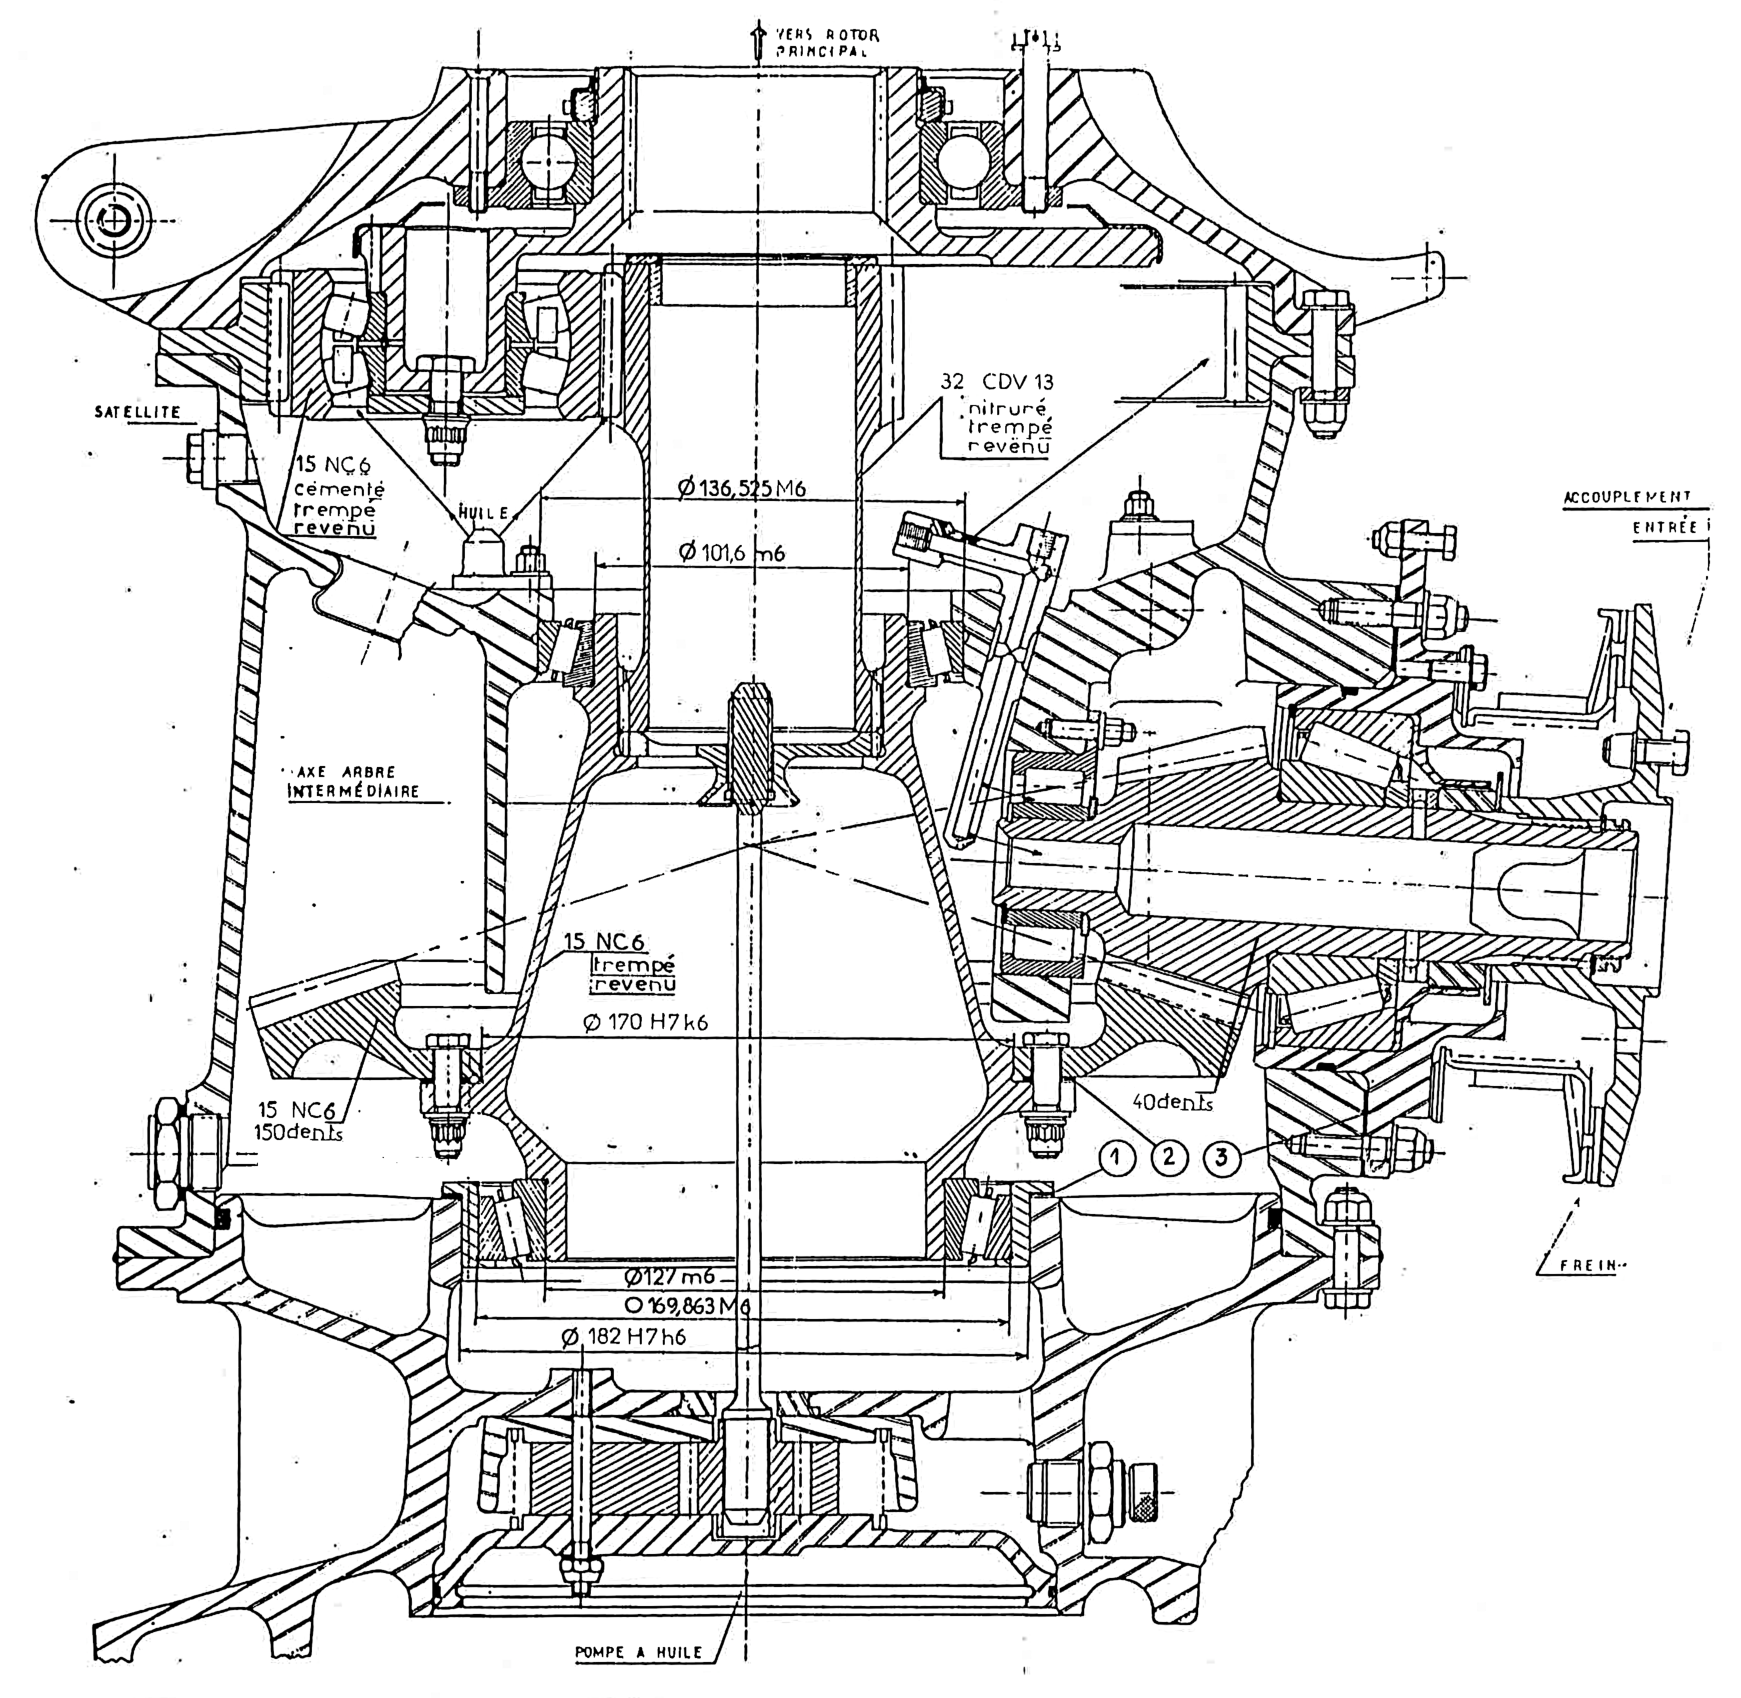
\includegraphics[width=\linewidth]{img/Hélico/transmission_plan.pdf} 
\end{center}
}{\begin{center}
 \includegraphics[width=\linewidth]{img/Hélico/transmission_plan_cor.png}
 \end{center}
}

\reponse{6}{}{\begin{center}
 \def\svgwidth{.8\linewidth}
 \input{img/Hélico/graphe_liaisons.pdf_tex}
\end{center}}


\reponse{10}{}{\begin{center}
 \def\svgwidth{.8\linewidth}
 \input{img/Hélico/schema_cinematique.pdf_tex}
\end{center}}

\reponse{5}{}{
$\omega_{pal}=\omega_{ps}$

Formule de Willis $\dfrac{\omega_{c}-\omega_{ps}}{\omega_{p}-\omega_{ps}}=-\dfrac{22}{75}$

Avec $\omega_{c}=0$, donc $\dfrac{\omega_{ps}}{\omega_{p}-\omega_{ps}}=\dfrac{22}{75}$

$\omega_{ps}=\dfrac{22}{75}\cdot (\omega_{p}-\omega_{ps})$

$\omega_{ps}\cdot (1+\dfrac{22}{75})=\dfrac{22}{75}\cdot \omega_{p}$

$\dfrac{\omega_{ps}}{\omega_{p}}=\dfrac{\dfrac{22}{75}}{(1+\dfrac{22}{75})}=\dfrac{22}{22+75}=\dfrac{22}{97}\approx 0,2$

$\dfrac{\omega{p}}{\omega_{mot}}=\dfrac{40}{150}\approx 0,25$, donc $\dfrac{\omega_{pal}}{\omega_{mot}}=0,05$.
}

\end{document}